\documentclass[border=10pt]{standalone}
\usepackage{pgfplots}
\pgfplotsset{compat=1.18}
\begin{document}
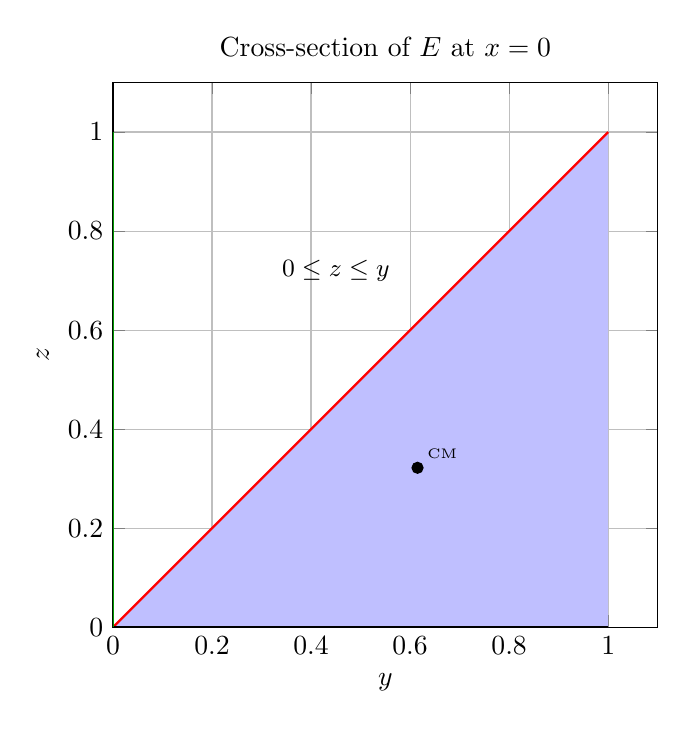
\begin{tikzpicture}
\begin{axis}[
    xlabel=$y$, ylabel=$z$,
    width=8.5cm,height=8.5cm,
    xmin=0,xmax=1.1,ymin=0,ymax=1.1,
    axis equal image,
    grid=both,
    title={Cross-section of $E$ at $x=0$}]
\addplot[fill=blue!25, draw=none] coordinates {(0,0)(1,1)(1,0)} \closedcycle;
\addplot[red, thick, domain=0:1]{x};
\addplot[black, thick, domain=0:1]{0};
\addplot[green!60!black, thick] coordinates {(0,0)(0,1)};
\addplot[only marks, mark=*, mark size=2pt] coordinates {(0.615,0.322)};
\node at (axis cs:0.615,0.322)[above right,font=\tiny]{CM};
\node[font=\small] at (axis cs:0.45,0.72){$0\leq z\leq y$};
\end{axis}
\end{tikzpicture}
\end{document}